\section{Maquetas}
A partir de toda la información reunida, hemos desarollado una maqueta de la interfaz de la aplicación. Se ha hecho a traves del IDE de NetBeans para que sea mas parecida al producto final. Solamente se mostrará de la parte del empleado, supóngase que la parte del gerente tendrá un aspecto muy parecido.\\

En primer lugar, el usuario sera bienvenido con la siguiente pantalla:\\
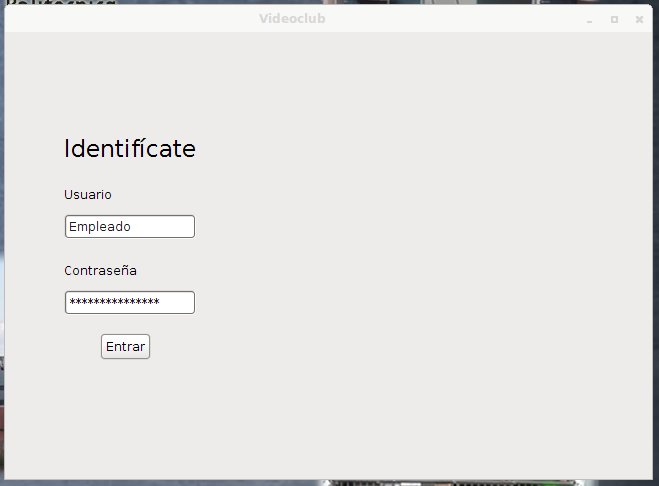
\includegraphics[width=10cm, height=10cm, keepaspectratio]{img/inicio.jpg}\\

Si el empleado quiere alquilar una película:\\
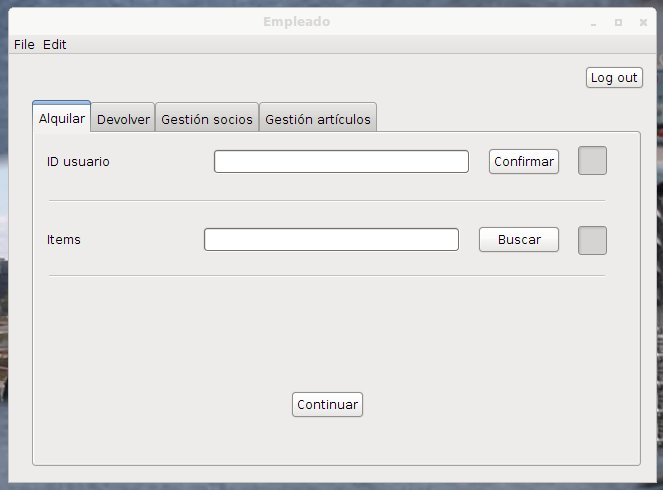
\includegraphics[width=10cm, height=10cm, keepaspectratio]{img/empleado-alquilar.jpg}\\
\clearpage

Primero ingresa la UID del socio. Luego, cuando el empleado busca el artículo, aparece la ventana de búsquedas:\\
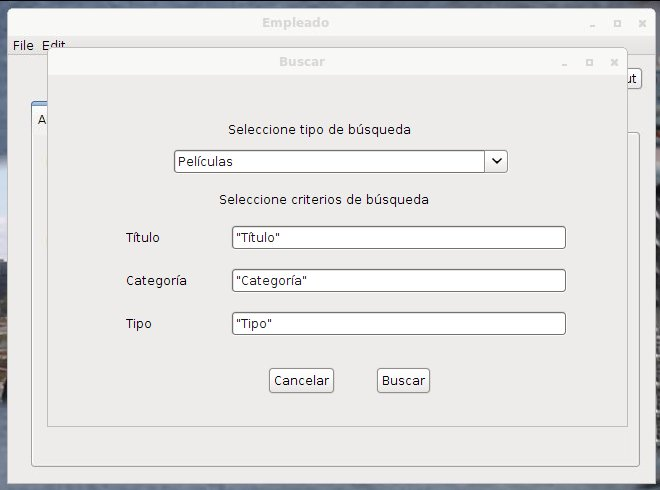
\includegraphics[width=10cm, height=10cm, keepaspectratio]{img/buscar-entrada.jpg}\\

Cuando el empleado tiene todos los datos de alquiler y le da a continuar, aparece la ventana de pago. En ella hay que seleccionar el método de pago:\\
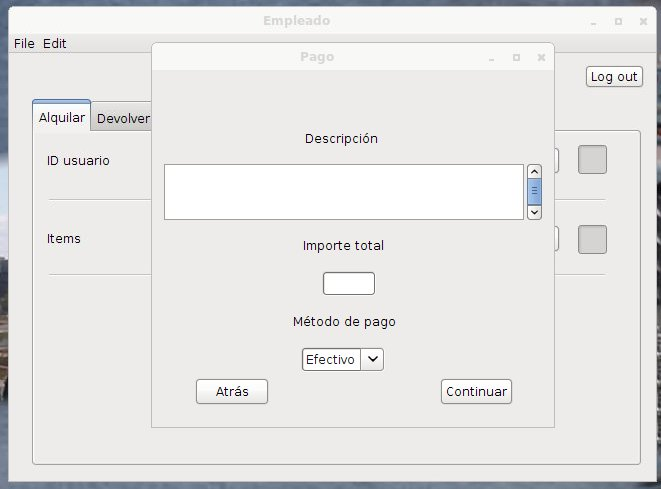
\includegraphics[width=10cm, height=10cm, keepaspectratio]{img/pagar.jpg}\\
\clearpage

Si el empleado quiere devolver una película, el menú será muy parecido al de alquiler:\\
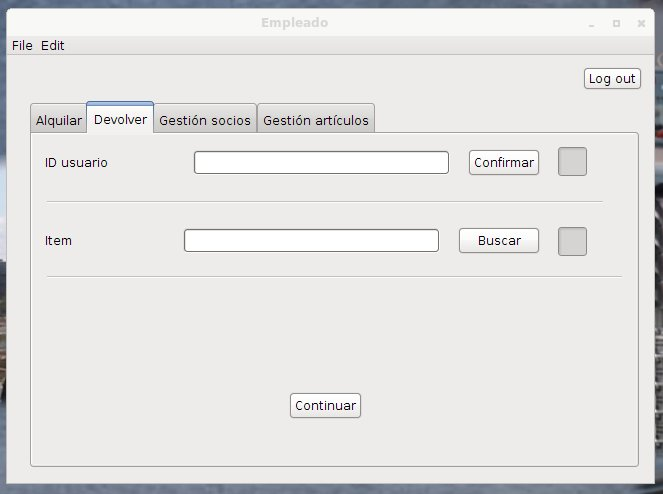
\includegraphics[width=10cm, height=10cm, keepaspectratio]{img/empleado-devolver.jpg}\\

Si el empleado accede a la gestión de socios, podrá dar de alta o de baja a socios, y contratar tarifas VIP:\\
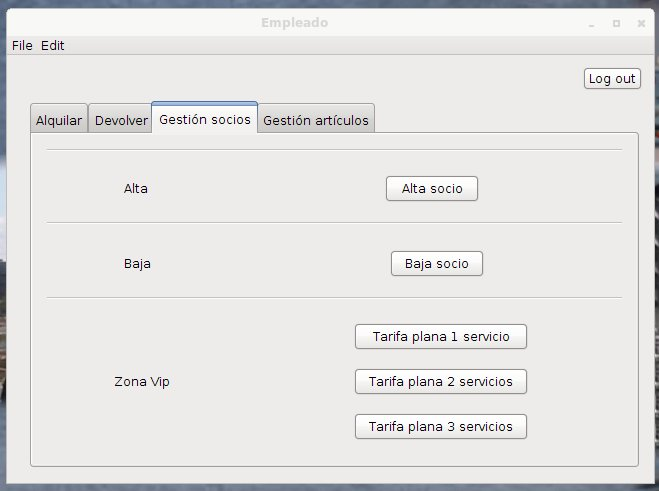
\includegraphics[width=10cm, height=10cm, keepaspectratio]{img/empleado-socios.jpg}\\
\clearpage

Si por ejemplo quiere dar de alta a un usuario, saldrá la siguiente ventana:\\
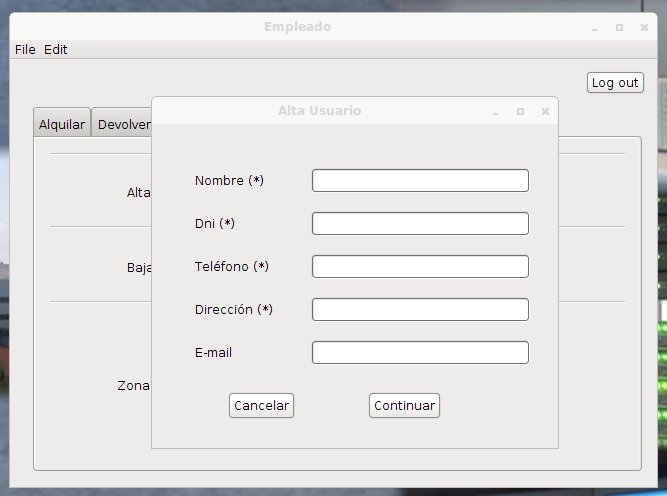
\includegraphics[width=10cm, height=10cm, keepaspectratio]{img/altasocio.jpg}\\

Si el empleado accede a la gestión de artículos, podrá añadir nuevos artículos y retirar alguno ya existente (aquí tambien podrá acceder el gerente):\\
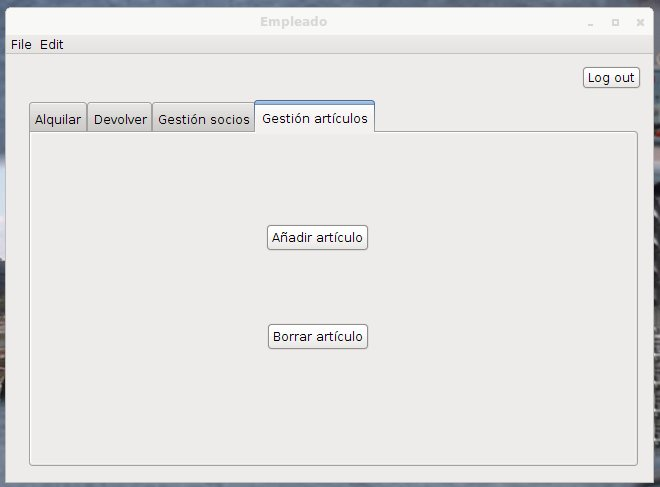
\includegraphics[width=10cm, height=10cm, keepaspectratio]{img/empleado-articulos.jpg}
\clearpage

Si el empleado quiere añadir un artículo al videoclub, saldrá la siguiente ventana:\\
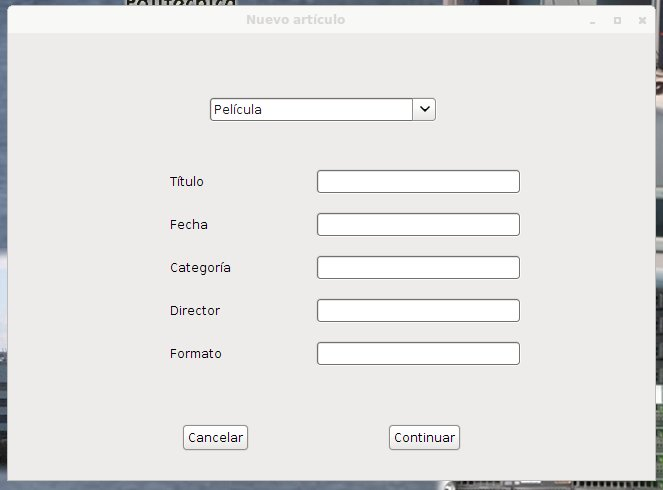
\includegraphics[width=10cm, height=10cm, keepaspectratio]{img/nuevoarticulo.jpg}\\
\clearpage

	
